\documentclass[tikz,border=10pt]{standalone}
\usetikzlibrary{calc}
\begin{document}
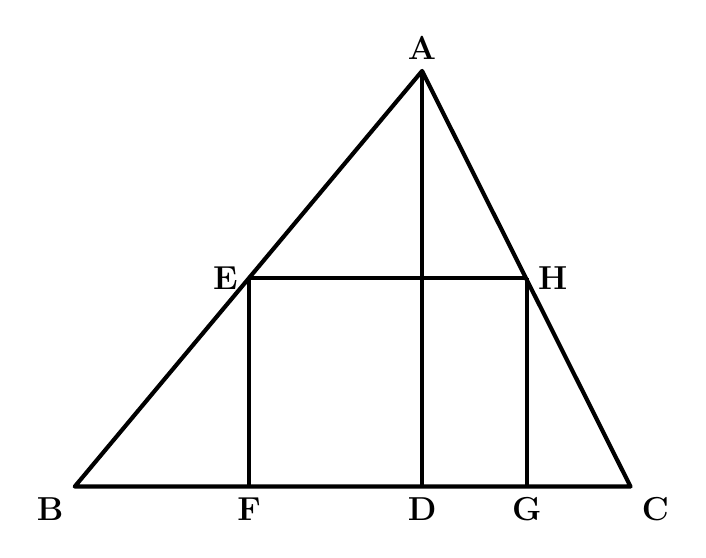
\begin{tikzpicture}[line width=1.5pt, line join=round, font=\fontsize{12}{14.4}\selectfont]
  % Coordinates: origin at D(364,420) px, scale 0.014953 cm/px, y flipped
  \coordinate (A) at (0,5.278);
  \coordinate (B) at (-4.411,0);
  \coordinate (C) at (2.647,0);
  \coordinate (D) at (0,0);
  \coordinate (E) at (-2.198,2.647);
  \coordinate (F) at (-2.198,0);
  \coordinate (G) at (1.331,0);
  \coordinate (H) at (1.331,2.647);

  % Triangle sides and altitude AD use the global 1.5pt width
  \draw (A) -- (B) -- (C) -- cycle;
  \draw (A) -- (D);

  % Rectangle sides use the same global 1.5pt width
  \draw (E) -- (H);
  \draw (E) -- (F);
  \draw (H) -- (G);

  % Point labels: unchanged from v1
  \node[above] at (A) {$\mathbf{A}$};
  \node[below left] at (B) {$\mathbf{B}$};
  \node[below right] at (C) {$\mathbf{C}$};
  \node[below] at (D) {$\mathbf{D}$};
  \node[left] at (E) {$\mathbf{E}$};
  \node[below] at (F) {$\mathbf{F}$};
  \node[below] at (G) {$\mathbf{G}$};
  \node[right] at (H) {$\mathbf{H}$};
\end{tikzpicture}
\end{document}